\documentclass[conference]{IEEEtran}

\usepackage{cite}
\usepackage{url}
\usepackage[cmex10]{amsmath}
\usepackage[ruled]{algorithm2e}
\usepackage{algorithmic}
\usepackage{amssymb}
\usepackage{multirow}
\interdisplaylinepenalty=2500

% *** GRAPHICS RELATED PACKAGES ***
%

% % % % % MACROS  % % % % % % %
\newcommand{\imagepath}{../../images/external/location_routing}
\newcommand{\colwidth}{2.6in}
% % % % % % % % % % % % % % % %

\ifCLASSINFOpdf
  \usepackage[pdftex]{graphicx}
  % declare the path(s) where your graphic files are
  % ../.. is the GeocronDocuments directory
\graphicspath{{../../images/diagrams/}{../../images/external/location_routing/}{../../images/plots/}}
  % and their extensions so you won't have to specify these with
  % every instance of \includegraphics
  \DeclareGraphicsExtensions{.pdf,.png}
\else
  % or other class option (dvipsone, dvipdf, if not using dvips). graphicx
  % will default to the driver specified in the system graphics.cfg if no
  % driver is specified.
  % \usepackage[dvips]{graphicx}
  % declare the path(s) where your graphic files are
  % \graphicspath{{../eps/}}
  % and their extensions so you won't have to specify these with
  % every instance of \includegraphics
  % \DeclareGraphicsExtensions{.eps}
\fi
\usepackage[caption=false,font=footnotesize]{subfig}
\hyphenation{op-tical net-works semi-conduc-tor}
\begin{document}
%
% can use linebreaks \\ within to get better formatting as desired
\title{CS237 Project final report}

\author{\IEEEauthorblockN{Kyle E. Benson and Zhipeng Huang}
\IEEEauthorblockA{Donald Bren School of Information and Computer Sciences\\
University of California, Irvine\\
Irvine, California 92697\\
Email: kebenson@uci.edu, zhipengh@uci.edu}}

% use for special paper notices
\IEEEspecialpapernotice{(Project Report for CS 237 - Distributed Systems Middleware)}

\maketitle

\section{Introduction}


With the increasing availability and decreasing cost of microelectromechanical systems (MEMS) sensors, several projects have begun exploring the use of these devices in Internet-connected distributed sensing efforts.
The Quake-Catcher Network \cite{qcn} and Community Seismic Network \cite{csn_site} utilize small inexpensive accelerometers attached to volunteers' computers to monitor seismic activity.
When they detect abnormal ground motion, indicative of a possible seismic event, these hosts report to a central server that processes the information and determines if an earthquake has occurred.
Other such devices, whose information could help understand regional impact of phenomena, include weather stations, pollution detectors, and geiger counters \cite{caltech_sensors}.

We believe that the domain of disaster response could benefit from the inputs of these community scale networked sensors.
Such sensor networks could potentially detect these events' onset and warn possibly affected individuals to find shelter, as well as aid first responders through increased situational awareness.
However, network failures can severely hamper these networks' ability to gather useful information in a timely manner, especially important for those aimed at monitoring fast-moving destructive physical phenomena such as earthquakes and floods.
Such events often result in large-scale geographically correlated failures in addition to serious network congestion as individuals contact each other or request help, exacerbating failures or tying up channels entirely.

Many previous projects have explored resilience to failures in the Internet, although few have addressed large-scale geographically correlated failures.
Most of these works aim to formally model failures and identify strategies for designing more reliable network infrastructure.
For example, \cite{geocorrelated} studied regional failures by defining line segments that cut any intersecting links in the graph representative of the network topology under consideration.
Some of the most devastatingly impacting link cuts possible in a particular network provider were identified and categorized in \cite{net_disaster_planning} to aid in planning more resilient networks.
Both \cite{model_analysis} and \cite{resilience_survey} discuss general challenges to networked systems and discuss the proposed \emph{ResiliNets} framework, which aims to formalize the steps and strategies involved in designing and maintaining more robust networks.


\begin{figure}[!t]
\centering
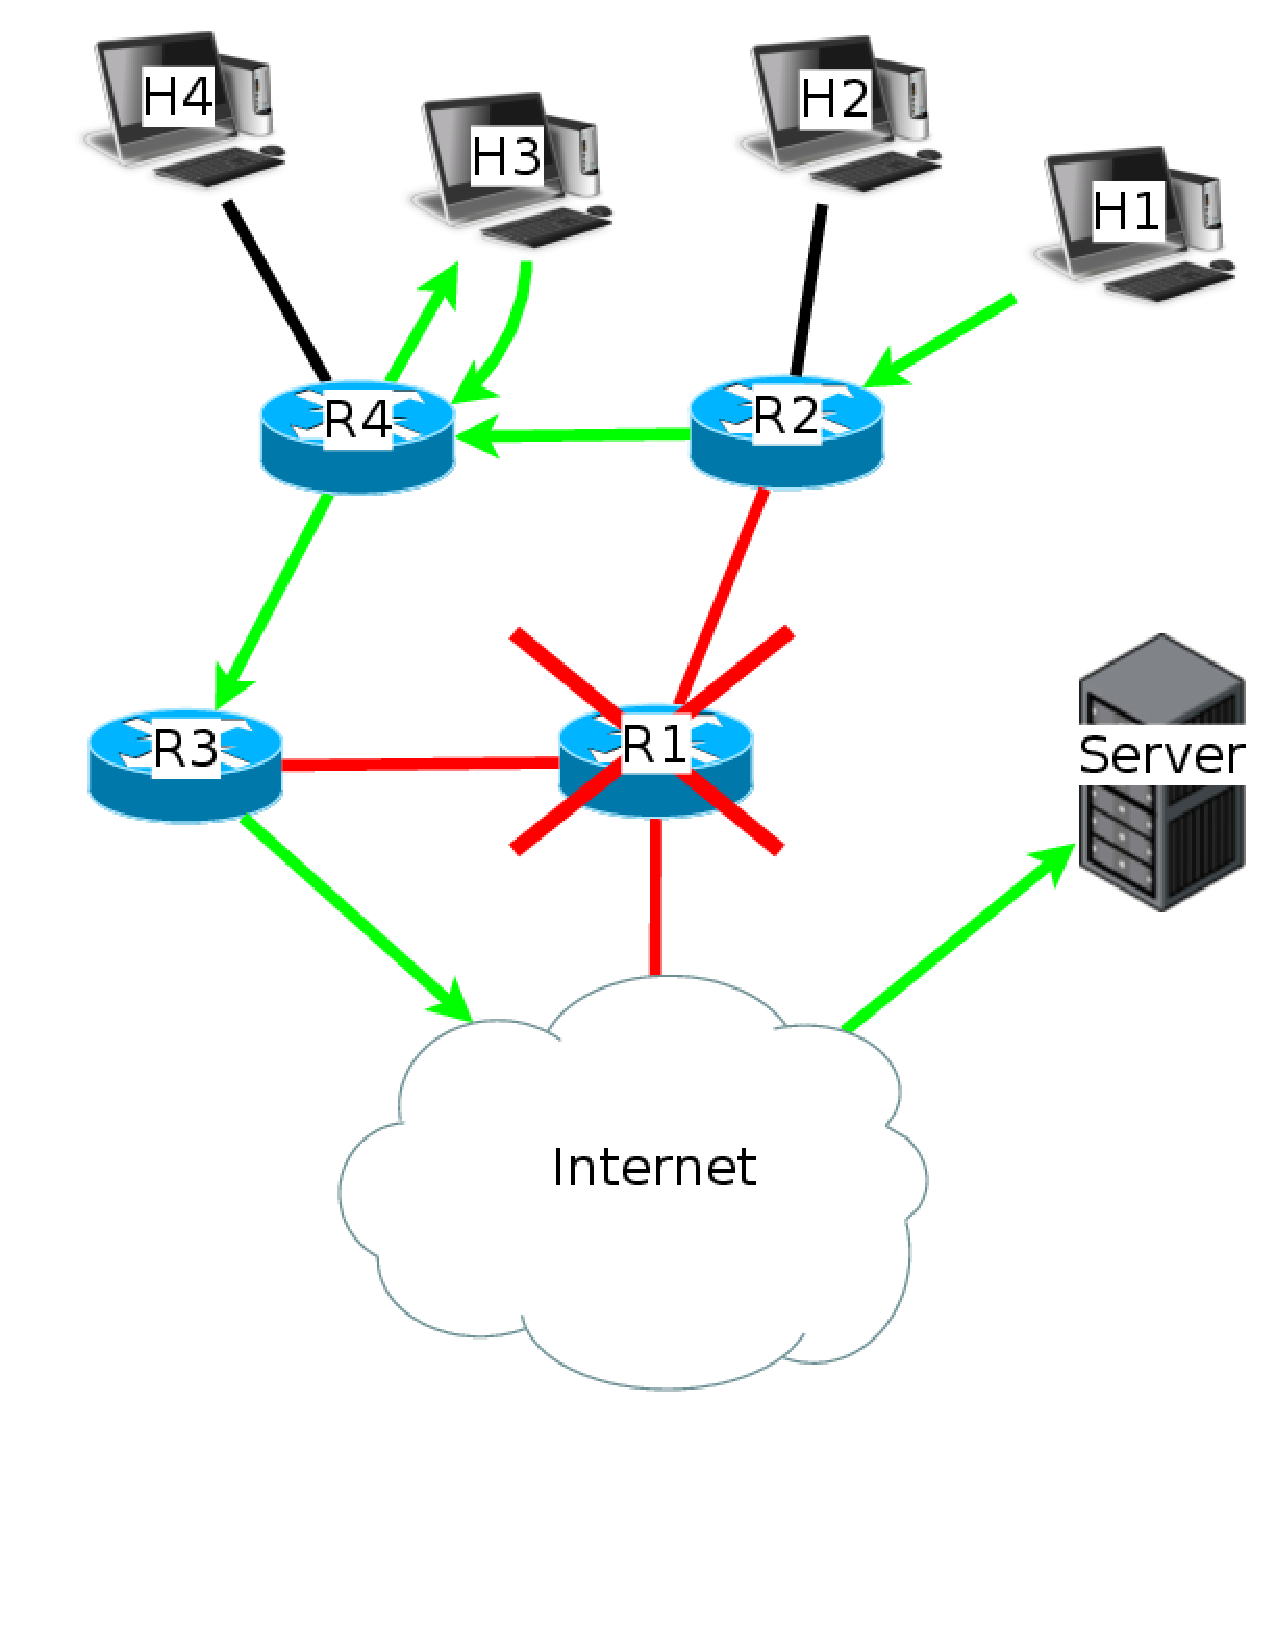
\includegraphics[width=2.5in]{overlay_path.pdf}
\caption{An overlay routing example.  Consider R1, R2, R3, and R4 are routers.  R1 (crossed out) has failed and host H1's normal (shortest) path to the server is unavailable.  Instead, it can route through nearby nodes in the order shown (R2, R4, H3, R4, R3, through the Internet and finally to the server).  H3 serves as an intermediary hop so that H1 can target a different path along the underlying network, without the network knowing about it.}
\label{fig_overlay_path}
\end{figure}

\subsection{Resilient Overlay Networks}

In this paper, we explore the creation and use of resilient overlay networks (RONs) to address large-scale disasters and the resultant failures that hamper sensor devices', as well as responders', ability to deliver data over the Internet backbone.
Previous research \cite{ron,reactive_routing} has shown that these overlay networks can help route packets along alternative communication paths when the primary one is damaged, unavailable, or simply congested.
This particularly helps while routing protocols still have not converged and established new end-to-end paths.

%TODO: find the 40 seconds to SON speaker on 11/1 was referring to

When a particular link becomes unavailable, whether due to a physical failure or congestion, the network's underlying routing protocols may take several minutes to find an alternative route.
Several case studies have identified serious problems with routing over the Internet, such as \cite{routing_resilience_analysis} that discovered several paths hopping to other continents unnecessarily after a major earthquake in Taiwan.
This paper also determined that BGP policies significantly reduced Internet resilience due to disallowing certain paths.
Most visible failures were found to not exceed 5-15 minutes in \cite{reactive_routing} and BGP route update convergence was found to take up to 15 minutes after a fault in \cite{route_convergence}.
During this time, some end-to-end connections may be unavailable because certain paths are non-functional but others may exist that the routing infrastructure is not yet aware of.

%TODO: 6 hours of downtime from that speaker

In RONs, routers try to find an alternative path when the main one fails to deliver a packet, as shown in Figure \ref{fig_overlay_path}.
They attempt to make contact with another node in the overlay to see if that node is reachable and has a working path to the desired destination.
If it does, then the traffic is routed through this intermediate node to the destination until a more direct path becomes available or less congested.
Adding this level of intelligence to the routing infrastructure may incur large amounts of additional complexity and cost, but it can also be accomplished with simple end hosts in a peer-to-peer-like fashion.
Deploying end hosts for the specific purpose of establishing a RON, or using those that are already part of a distributed sensing effort for this purpose as well, could possibly increase the reliability of a system without having to modify any of the routers in the underlying physical network.

\subsection{Contribution}
To lend focus to our work, we explored this problem in the context of CSN \cite{csn_site}.
In order to effectively identify and categorize earthquakes in a timely manner, the small messages sent by the seismic sensors, referred to as \emph{picks}, must arrive at the server for analysis within a few seconds at most, especially if CSN is to be used as any sort of early warning system.
One expects possible disruptions of the telecommunications infrastructure during a powerful seismic event and so this scenario seemed a perfect application for our technique.

This paper builds upon previous work \cite{Benson2013}, extending the GeoCRON simulator to compare new heuristics on different topologies.
In the following sections, we first describe the changes made to support the new BRITE topology generator, the heuristics implemented in the simulator, and the results from the simulations we ran.

%%%%%%%%%%%%%%%%%%%%%%%%%%%%%%%%%%%%%%%%%%%%%%%%%%%%%%%%%%%%%%%%%%%%%%%%%%%%%%%%%%%%%%%

\section{Topology Generator}

In order to better compare the location routing heuristics, we wanted to generate topologies with more fine-grained information than is available with the currently-used Rocketfuel topologies.
This allows nodes within a particular region to have different locations, opening up more possibilities for diverse path choices.

For this project, we made some large changes to the simulator in order to support the BRITE topology generator, which is integrated into ns-3.
To accomplish this, we first had to reorganize the way in which the experiments are set up and run.
Specifically, we modified the main core of the GeoCRON simulator to first build a network of nodes with static positions, then index the nodes based on location before finally installing applications and running the simulations.
This allows us to plug in new topology generators as long as they set positions for each node.

Because the topology generator has to set the nodes' positions, we had to extend the BRITE topology generator to do so.
Once this was done and the experiment core was refactored, plugging in the BRITE model was simple.
This change also allows us to plug in simpler topology generators, such as grids or stars, and even more complex ones, such as Inet.

%%%%%%%%%%%%%%%%%%%%%%%%%%%%%%%%%%%%%%%%%%%%%%%%%%%%%%%%%%%%%%%%%%%%%%%%%%%%%%%%%%%%%%% 

\section{Algorithm}
There are six routing heuristic algorithms that have been tested and compared in the simulation: orthogonal distant path heuristic, new region heuristic, new angle path heuristic, distant-dependent path heuristic, furthest first path heuristic and closest first path heuristic.
The New Angle, Distance-Dependent, and Furthest-First heuristics are new contributions from this project.
\subsection{Orthogonal Distant Path Heuristic}
The intuition of this heuristic is to avoid the straight path, without diverging from it too much.  It strikes a middle ground by choosing a path at an ideal angle of $45^{\circ}$, which makes the angle at the top orthogonal, hence the name.
\begin{algorithm}
\DontPrintSemicolon
\SetKwBlock{Begin}{begin}{end}
\SetAlgoLined
\SetAlgoLongEnd
\scriptsize
\Begin{
\tcc*[l]{Sensor, overlay and server node are a, c, b respectively}
$idealDist = |0.5 \cdot dist(a,b)|$\;
$perpDist = |\sin (angA) \cdot dist(a,c)|$\;
\lIf{$angA > \frac{\pi}{2}$ {\bf or} $angA + angC < \frac{\pi}{2}$ {\bf or} $perpDist > dist(a,b)$} {$likelihood = 0$\;}
\lElse {$likelihood = 0.5 \cdot (( 1.0 - (||perpDist|-|idealDist|| / idealDist)^{2}) + ( 1.0 - (|\frac{\pi}{2} - angC| / \frac{\pi}{2})^{2}))$\;}
}
\caption{}
\small
\end{algorithm}

% % % % % % % % %
%
\subsection{New Region Heuristic}
The intuition of this heuristic is to avoid regions that have been previously attempted unsuccessfully.  We assume that no further attempts to contact such a region will succeed.
\begin{algorithm}
\DontPrintSemicolon
\SetKwBlock{Begin}{begin}{end}
\SetAlgoLined
\SetAlgoLongEnd
\scriptsize
\Begin{
%\tcc*[l]{Discover any node that has not been discoverd in this region}
\lIf{$peer.region \in regionsAttempted$} {$likelihood = 0$\;}
\lElse {$likelihood = 1.0$\;}
}
\caption{}
\small
\end{algorithm}

% % %
%
\subsection{New Angle Path Heuristic}
This heuristic attempts paths along new angles different from the ones previously attempted.
\begin{algorithm}
\DontPrintSemicolon
\SetKwBlock{Begin}{begin}{end}
\SetAlgoLined
\SetAlgoLongEnd
\scriptsize
\Begin{
%\tcc*[l]{The angle could be either acute or obtuse.}
$angle = Angle(overlay,server)$\;
\lIf{$angle = \pi$ {\bf or} $angle = 0$} {$initLikelihood = 0$\;}
\lElseIf{$angle < \pi$} {$initLikelihood = \cos (angle - \frac{\pi}{4})$\;}
\lElseIf{$angle > \pi$} {$initLikelihood = \cos (2 \cdot ((2\pi - angle) - \frac{\pi}{4})/3)$\;}
\lForEach {$path \in pathsAttempted$} {$thisLikelihood = |\frac{\sin (angle)}{2}|$\;} {$newLikelihood *= thisLikelihood$\;}
%\tcc*[l]{aggregate likelihoods to make punishments on wrong choices}
}
\caption{}
\small
\end{algorithm}

% % % %
%
\subsection{Distance-Dependent Path Heuristic}
This heuristic attempts paths that use overlay nodes at an ideal distance from the sensor.  This ideal distance is chosen as a radius that reaches half-way to the server.
\begin{algorithm}
\DontPrintSemicolon
\SetKwBlock{Begin}{begin}{end}
\SetAlgoLined
\SetAlgoLongEnd
\scriptsize
%\SetAlgoSkip{bigskip}
%\SetAlgoInsideSkip{medskip}
%$/*Initialization*/$\;
\Begin{
\tcc*[l]{minDist = some reasonably small number}
$idealDist = 0.5 \cdot dist(sensor,server)$
$dist = dist(sensor,overlay)$
\lIf{$dist <= minDist$} {$likelihood = 0$\;}
\lElseIf{$minDist < dist < idealDist$} {$likelihood = dist^{2} / idealDist^{2}$\;}
\lElseIf{$dist >= idealDist$} {$likelihood = idealDist / dist $\;}
}
\caption{}
\small
\end{algorithm}

% % %
%
\subsection{Furthest First Path Heuristic}
Thus, this heuristic considers overlay peers located further away to be more likely candidates.
\begin{algorithm}
\DontPrintSemicolon
\SetKwBlock{Begin}{begin}{end}
\SetAlgoLined
\SetAlgoLongEnd
\scriptsize
\Begin{
\tcc*[l]{minDistance = some constant small number}
\lIf{$dist(a,b) < minDistance$} {$likelihood = 0$\;}
\lElse {$likelihood = (dist(a,b) - minDistance) / dist(a,b) $\;}
}
\small
\end{algorithm}

% % %
%
\subsection{Closest First Path Heuristic}
The intuition of this heuristic is to contact nearby overlay nodes that have found a path out of the local region.  We found, however, that this approach does not always work well in practice, likely due to the path similarity inherent with nearby nodes.
\begin{algorithm}
\DontPrintSemicolon
\SetKwBlock{Begin}{begin}{end}
\SetAlgoLined
\SetAlgoLongEnd
\scriptsize
\Begin{
\tcc*[l]{maxDistance = some constant large number}
\lIf{$dist(a,b) > maxDistance$} {$likelihood = 0$\;}
\lElse {$likelihood = (maxDistance - dist(a,b)) / maxDistance $\;}
}
\caption{}
\small
\end{algorithm}

% % %
%
\section{Conclusion}
In this paper, we described our recent additions to the GeoCRON simulator.
In particular, we:

\begin{itemize}
 \item Switched from Rocketfuel to BRITE for creating ns-3 network topologies
\item Added the New Angle heuristic, which repeatedly tries overlay nodes at diverse angles
\item Added the Furthest-First heuristic, which attempts to contact overlay nodes furthest from the source
\item Added the Distance-Dependent heuristic, which tries to pick overlay nodes at an ideal distance from the source, preferring nodes further away over those close by
\item Defined a new method for assigning regions to nodes in which the region of study is broken up into a grid, where each cell is a constant size
\end{itemize}

We ran simulations on topologies of 10,000 nodes and 25 regions, comparing the peformance of each heuristic with each other.
The results were inconclusive, demonstrating that further refinement and/or combinations of heuristics are necessary to improve the delivery ratio.
For example, the New Angle and Distance-Dependent heuristics may be combined with varying weights to pick nodes both far away from the source as well as along diverse paths.

There are certain other aspects that need to be improved in the future.
First of all, a detailed comparison between the six heuristics should be explored regarding aspects such as difference in convegence time, latency, expected delivery ratio, etc.
Moreover, the purpose of the simulation of the six algorithms should be more clear.

\end{document}